\section{A Taxonomy of LLM-Based Code Review}\label{sec:taxonomy}

Existing taxonomies are organised by task: 34 tasks in nine macro-categories~\cite{tufano2025automating}, or five domains and 18 tasks for benchmarks~\cite{khan2026survey}. None captures the system-level, cost and risk dimensions that dominate 2024--2026 work. We therefore classify each work on seven orthogonal dimensions, so that a paper occupies one cell per dimension (Fig.~\ref{fig:taxonomy}).

\begin{itemize}
\item \textbf{D1 Review task:} necessity estimation, comment generation, issue detection in PRs, refinement, comment classification, security review, static-analysis warning triage, multi-round review, and evaluation.
\item \textbf{D2 Model adaptation:} pre-training, full fine-tuning, PEFT, prompting, RAG, preference/RL, reasoning tuning, data-centric methods, and distillation.
\item \textbf{D3 System architecture:} single call, generator plus filter, multi-role agents, tool-using agents, static-analysis hybrids, multi-run aggregation, and routing.
\item \textbf{D4 Context scope:} hunk, function, file, repository, and non-code intent.
\item \textbf{D5 Evaluation regime:} text similarity, LLM judges, issue-level precision/recall, comprehension probes, tests, field outcomes, and controlled experiments.
\item \textbf{D6 Deployment and cost profile (new):} frontier API, self-hosted large model, small or local model, cascade or routing, and whether tokens, dollars or latency are reported.
\item \textbf{D7 Trust and risk treatment (new):} false-positive control, hallucination detection, adversarial robustness, human factors, and privacy.
\end{itemize}

D6 and D7 are the main additions. Cost and risk are already visible in the evidence: one industrial study reports a cost of about \$0.48 per PR together with a longer PR closure time~\cite{cihan2025automated}, hallucination detection has its own industrial method~\cite{tantithamthavorn2026hallujudge}, and attacks on real review pipelines~\cite{alexopoulos2026when,isbarov2026gitinject} and anchoring in a controlled experiment~\cite{tufano2025deep} are now documented.

Mapped onto this grid, the literature piles up in one region: comment generation or issue detection (D1), PEFT or prompting (D2), a single call or generator-plus-filter pipeline (D3), issue-level or field evaluation (D5), and frontier APIs (D6). Two regions are essentially empty: small or cascaded models evaluated on real-PR issue detection (D6 crossed with D5), and defences against adversarial attacks (D7), as opposed to the attacks themselves.

\begin{figure}[t]
\centering
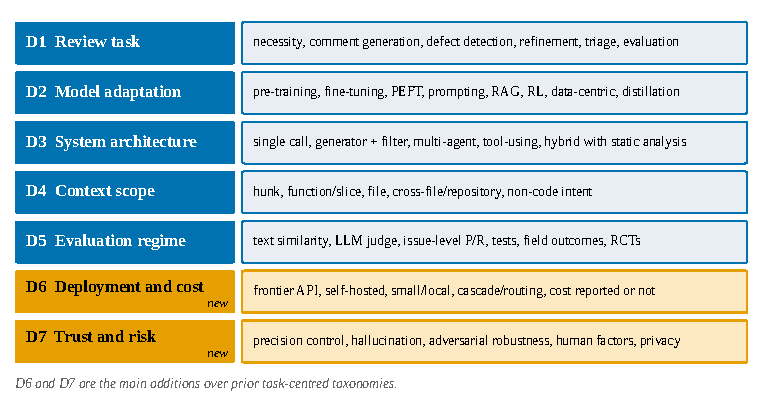
\includegraphics[width=\textwidth]{figures/taxonomy.pdf}
\caption{Proposed taxonomy: seven orthogonal dimensions (D1 review task, D2 model adaptation, D3 system architecture, D4 context scope, D5 evaluation regime, D6 deployment and cost profile, D7 trust and risk treatment) with their summarised categories. D6 and D7 are highlighted as additions over prior task-oriented taxonomies.}
\label{fig:taxonomy}
\end{figure}
